\documentclass[10pt, spanish, aspectratio=169]{beamer}

% --- Configuración de Idioma y Matemáticas ---
\usepackage[utf8]{inputenc}
\usepackage[spanish]{babel}
\usepackage{amsmath, amsfonts, amssymb}
\usepackage{graphicx}
\usepackage{booktabs}
\usepackage{hyperref}
\usepackage{subfigure}

% --- Tema Visual (Limpio y Profesional) ---
\usetheme{Madrid} 
\usecolortheme{whale} % Azul profesional
\setbeamertemplate{navigation symbols}{} % Quitar iconos feos de navegación

% --- Ruta de Imágenes ---
\graphicspath{{../doc/images/}}

% --- Metadatos ---
\title{Librería Python para CKKS en GPU}
\subtitle{Operaciones Tensoriales con Cifrado Homomórfico}
\author{Rafael Eduardo Contreras}
\institute{Universidad Central de Venezuela \\ Facultad de Ciencias}
\date{\today}

\begin{document}

% Portada
\begin{frame}
    \titlepage
\end{frame}

% Índice Automático
\begin{frame}{Contenido del Seminario}
    \tableofcontents
\end{frame}

% --- Carga de Secciones Modulares (26 slides en total) ---
% --- Part 1: Introduction & Motivation (Slides 1-3) ---
\section{Introducción y Motivación}

\begin{frame}{Título y Autores}
    \begin{center}
        \Huge \textbf{Librería Python para CKKS en GPU} \\
        \large \textit{Operaciones Tensoriales con Cifrado Homomórfico} \\
        \vspace{1cm}
        \normalsize \textbf{Rafael Eduardo Contreras} \\
        \textit{Universidad Central de Venezuela \\ Facultad de Ciencias}
    \end{center}
\end{frame}

\begin{frame}{El Dilema de la Privacidad}
    \begin{columns}
        \column{0.6\textwidth}
        \begin{itemize}
            \item Explosión del \textbf{Machine Learning (ML)} en áreas sensibles.
            \item \textbf{Sectores:} Medicina, Finanzas, etc.
            \item \textbf{Riesgo:} Fuga de datos al usar servicios de terceros en la nube para inferencia.
        \end{itemize}
        
        \column{0.4\textwidth}
        \begin{figure}
            \centering
            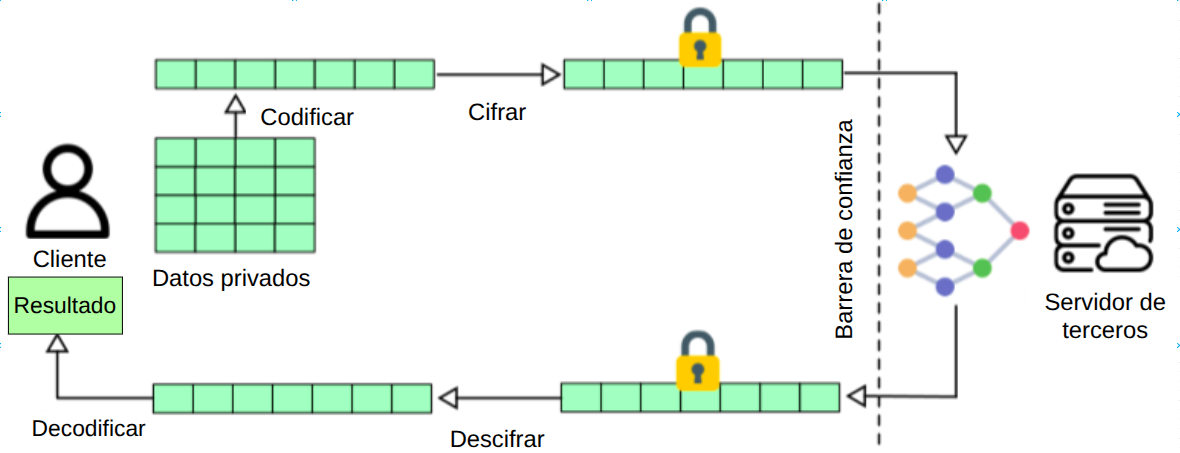
\includegraphics[width=\textwidth]{fhe_on_ml.png}
        \end{figure}
    \end{columns}
\end{frame}

\begin{frame}{Cifrado Homomórfico (HE) como Solución}
    \begin{itemize}
        \item \textbf{Definición:} Computar directamente sobre datos cifrados.
        \item \textbf{Propiedad:} El resultado, una vez descifrado, coincide con el obtenido en texto plano.
        \item \textbf{Beneficio:} El servidor nunca tiene acceso a la información sensible.
    \end{itemize}
\end{frame}

% --- Part 2: Fundamentals of HE & Modern Schemes (Slides 4-8) ---
\section{Fundamentos de HE}
\SectionFrame{Fundamentos de HE}

\begin{frame}{Orígenes y Evolución}
    \begin{itemize}
        \item \textbf{1978:} Rivest, Adleman y Dertouzos proponen \textit{"Privacy Homomorphisms"}.
        \[ E(m_1 \otimes m_2) = E(m_1) \otimes E(m_2) \]
        \item \textbf{Cifrado Parcialmente Homomórfico (PHE):}
        \begin{itemize}
            \item \textbf{RSA (Multiplicativo):}
            \[ c_1 \cdot c_2 = m_1^e \cdot m_2^e = (m_1 \cdot m_2)^e \pmod n \]
            \item \textbf{Paillier (Aditivo):}
            \[ g^{m_1} r_1^n \cdot g^{m_2} r_2^n = g^{m_1+m_2} (r_1 r_2)^n \pmod{n^2} \]
        \end{itemize}
    \end{itemize}
\end{frame}

\begin{frame}{Hacia el Cifrado Total (FHE)}
    \begin{itemize}
        \item \textbf{2009: Craig Gentry} presenta el primer esquema Totalmente Homomórfico (FHE).
        \item \textbf{Leveled FHE:} Esquemas diseñados para evaluar circuitos de una profundidad máxima predefinida.
        \item \textbf{Bootstrapping:} La gran innovación de Gentry.
        \begin{itemize}
            \item Proceso de "refresco" del texto cifrado para reducir el ruido.
            \item Evaluación homomórfica del propio circuito de descifrado.
        \end{itemize}
    \end{itemize}
    \vfill
    \begin{figure}
        \centering
        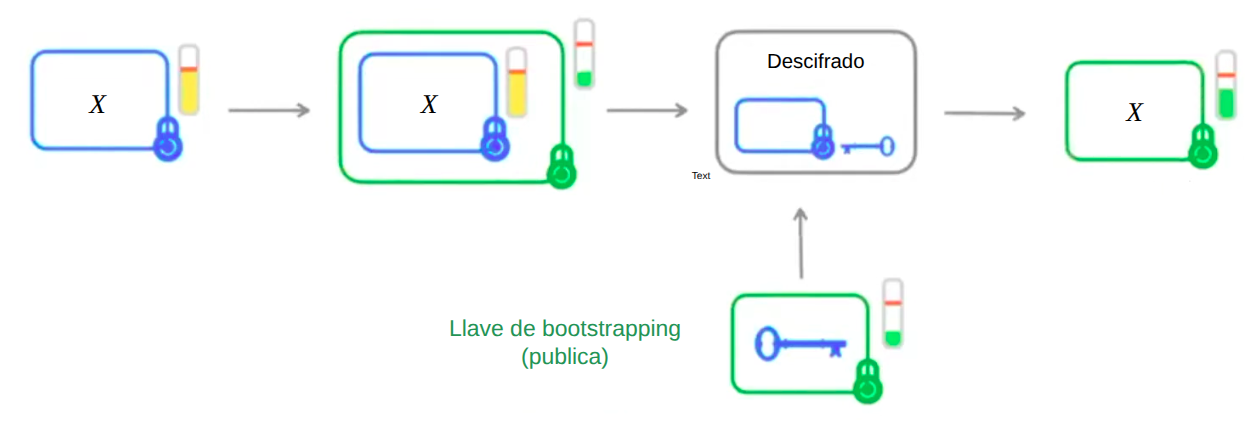
\includegraphics[width=0.6\textwidth]{bootstrap.png}
        \caption{Diagrama esquemático del proceso de Bootstrapping.}
    \end{figure}
\end{frame}

\begin{frame}{El Problema del "Ruido"}
    \begin{itemize}
        \item El cifrado incluye un "error" o ruido para garantizar seguridad.
        \item El ruido crece con cada operación homomórfica.
        \item La multiplicación aumenta el ruido mucho más rápido que la suma.
        \item Si el ruido supera un umbral, el descifrado falla.
    \end{itemize}
    \begin{center}
        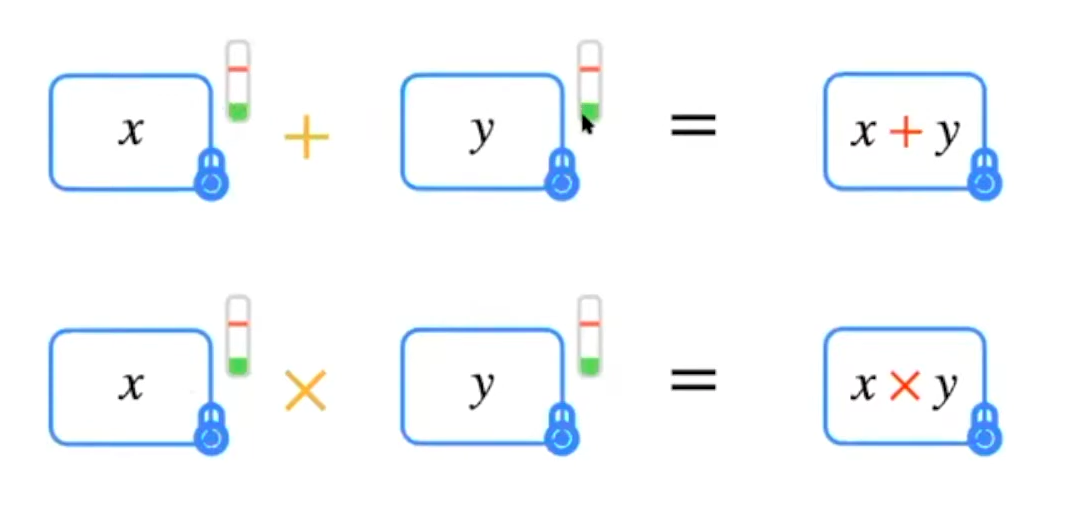
\includegraphics[width=0.6\textwidth]{noise.png}
    \end{center}
\end{frame}

\begin{frame}{Aprendizaje con Errores (LWE)}
    \begin{itemize}
        \item \textbf{Naturaleza:} Técnica asimétrica basada en problemas de retículos.
        \item \textbf{Clave Pública ($pk$):} Par $(\mathbf{A}, \mathbf{b})$ donde $\mathbf{b} = \mathbf{As} + \mathbf{e} \pmod q$.
    \end{itemize}
    
    \begin{block}{Ejemplo de Estructura}
        \[
        \underbrace{
        \begin{pmatrix} b_1 \\ b_2 \\ \vdots \\ b_m \end{pmatrix}
        }_{\mathbf{b} \in \mathbb{Z}_q^m}
        =
        \underbrace{
        \begin{pmatrix} 
        a_{11} & \dots & a_{1n} \\
        \vdots & \ddots & \vdots \\
        a_{m1} & \dots & a_{mn} 
        \end{pmatrix}
        }_{\mathbf{A} \in \mathbb{Z}_q^{m \times n}}
        \cdot
        \underbrace{
        \begin{pmatrix} s_1 \\ \vdots \\ s_n \end{pmatrix}
        }_{\mathbf{s} \in \mathbb{Z}_q^n}
        +
        \underbrace{
        \begin{pmatrix} e_1 \\ \vdots \\ e_m \end{pmatrix}
        }_{\mathbf{e} \in \chi^m} \pmod q
        \]
    \end{block}
    
    \begin{itemize}
        \item \textbf{Parámetros:} $n$ (seguridad), $m$ (muestras), $q$ (módulo), $\mathbf{e}$ (pequeño error).
    \end{itemize}
\end{frame}

\begin{frame}{Cifrado con LWE}
    Para cifrar un bit $m \in \{0, 1\}$ usando la clave pública $(\mathbf{A}, \mathbf{b})$:
    \begin{itemize}
        \item Seleccionar un vector aleatorio de muestreo $\mathbf{r}$.
        \item \textbf{Componentes del Criptograma $(c_1, c_2)$:}
        \[ \mathbf{c_1} = \mathbf{rA} \pmod q \]
        \[ c_2 = \mathbf{rb} + m\lfloor q/2 \rfloor \pmod q \]
        \item El mensaje se "esconde" desplazándolo a la mitad del módulo.
    \end{itemize}
\end{frame}

\begin{frame}{Descifrado con LWE}
    Para recuperar el mensaje $m$ usando la clave privada $\mathbf{s}$:
    \begin{itemize}
        \item \textbf{Operación de Descifrado:}
        \[ \mu = c_2 - \langle \mathbf{c_1}, \mathbf{s} \rangle \pmod q \]
        \item \textbf{Decisión:}
        \[ m = 
        \begin{cases} 
        0 & \text{si } \mu \text{ está más cerca de } 0 \\
        1 & \text{si } \mu \text{ está más cerca de } q/2 
        \end{cases} \]
        \item El descifrado es exitoso si el ruido acumulado es pequeño.
    \end{itemize}
\end{frame}

\begin{frame}{Aprendizaje con Errores en Anillos (RLWE)}
    El problema RLWE es una variante algebraica de LWE que traslada las operaciones de vectores y matrices a anillos de polinomios, donde la seguridad reside en la dificultad de distinguir muestras ruidosas de muestras aleatorias uniformes en el anillo.

    \begin{itemize}
        \item \textbf{Estructura:} Definido sobre el anillo $R_q = \mathbb{Z}_q[x] / \langle x^n + 1 \rangle$.
        \item \textbf{Ventajas:}
        \begin{itemize}
            \item Mayor eficiencia: Multiplicación vía \textbf{NTT}.
            \item Estructura compacta: Claves y textos cifrados más pequeños.
            \item Habilita operaciones paralelas nativas (\textbf{SIMD}).
        \end{itemize}
    \end{itemize}
\end{frame}

\begin{frame}{Esquemas FHE Modernos (Comparativa)}
    \begin{table}
        \centering
        \resizebox{\textwidth}{!}{
        \begin{tabular}{|l|l|l|l|}
            \hline
            \textbf{Característica} & \textbf{BGV / BFV} & \textbf{CKKS} & \textbf{TFHE} \\ \hline
            \textbf{Tipo de Dato} & Enteros exactos & Reales / Complejos & Bits / Enteros cortos \\ \hline
            \textbf{Gestión de Ruido} & Modulus/Scale switching & Reescalado & Bootstrapping rápido \\ \hline
            \textbf{Unidad de Cómputo} & Vectores (SIMD) & Vectores (SIMD) & Puertas Lógicas / LUT \\ \hline
            \textbf{Precisión} & Absoluta & Aproximada & Absoluta (Binaria) \\ \hline
        \end{tabular}
        }
    \end{table}
    \vfill
    \begin{itemize}
        \item \textbf{CKKS:} Seleccionado para este trabajo por su soporte nativo de aritmética aproximada, ideal para Redes Neuronales.
    \end{itemize}
\end{frame}

% --- Part 3: The CKKS Scheme in Depth (Slides 9-13) ---
\section{El Esquema CKKS}

\begin{frame}{Introducción al Esquema CKKS}
    Propuesto por Cheon, Kim, Kim y Song en 2017, el esquema CKKS representa un avance fundamental diseñado específicamente para el cómputo sobre números reales y complejos.

    \begin{itemize}
        \item \textbf{Propósito:} Habilitar aritmética aproximada de punto flotante de manera homomórfica.
        \item \textbf{Innovación:} Trata el ruido inherente del cifrado como un error de redondeo controlado, similar al cálculo numérico estándar.
        \item \textbf{Aplicabilidad:} Es el esquema de elección para tareas de Machine Learning y procesamiento de señales debido a su eficiencia en operaciones de alta precisión.
    \end{itemize}
\end{frame}

\begin{frame}{Parámetros Críticos en CKKS}
    \begin{itemize}
        \item \textbf{Grado del Polinomio ($N$):} Define el número de ranuras y el nivel de seguridad.
        \item \textbf{Módulo ($Q$):} Determina el "presupuesto de ruido" para operaciones.
        \item \textbf{Factor de Escala ($\Delta$):} Define la precisión de la representación decimal.
    \end{itemize}
\end{frame}

\begin{frame}{Codificación y SIMD}
    \begin{itemize}
        \item Inmersión Canónica para empaquetar $N/2$ números en un solo polinomio.
        \item Ventaja SIMD (\textit{Single Instruction, Multiple Data}).
        \item Una operación homomórfica afecta a todo el vector simultáneamente.
    \end{itemize}
    \begin{center}
        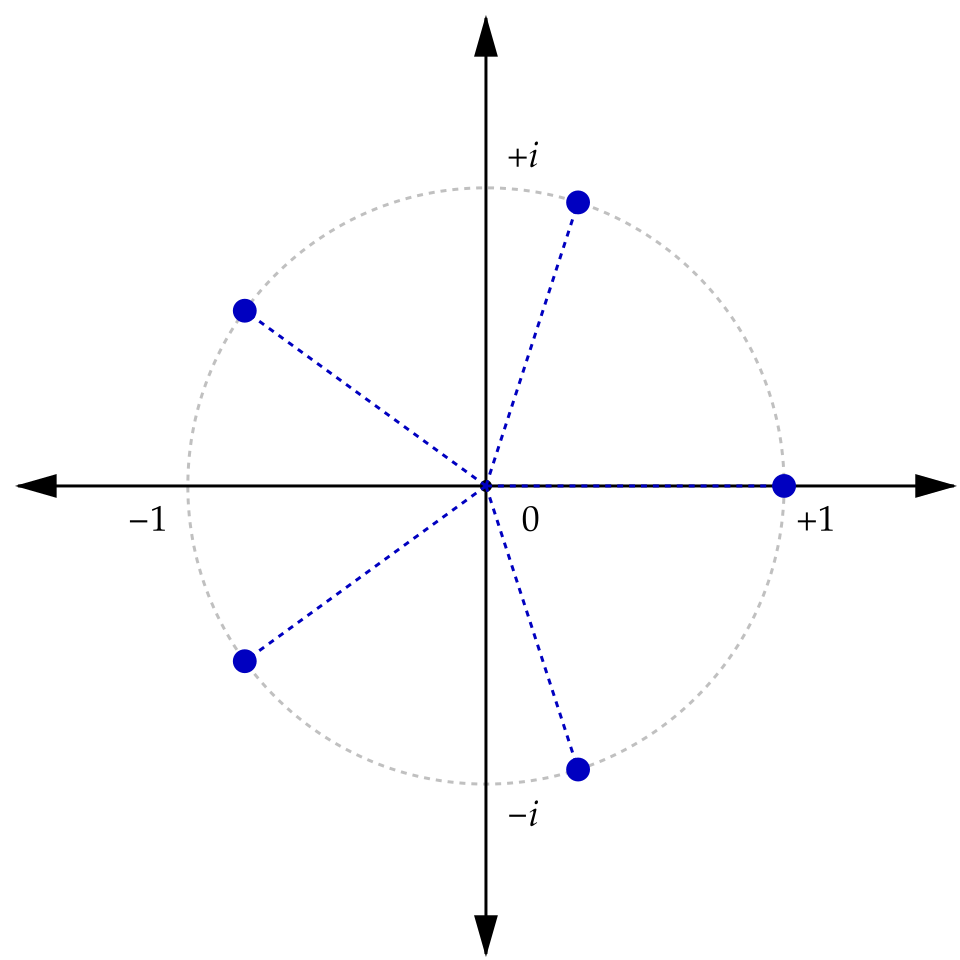
\includegraphics[width=0.4\textwidth]{roots_unity.png}
    \end{center}
\end{frame}

\begin{frame}{CKKS por Niveles (Leveled)}
    \begin{itemize}
        \item Cadena de módulos: $Q_L > Q_{L-1} > \dots > Q_0$.
        \item \textbf{Reescalado:} Reduce el módulo para gestionar el ruido tras multiplicaciones.
        \item Permite configurar parámetros para circuitos de profundidad fija.
    \end{itemize}
\end{frame}

\begin{frame}{Bootstrapping en CKKS}
    \begin{itemize}
        \item Evaluación homomórfica del circuito de descifrado.
        \item Refresco del texto cifrado para reducir el ruido acumulado.
        \item Permite realizar un número arbitrario de operaciones (FHE).
    \end{itemize}
    \vfill
    \begin{figure}
        \centering
        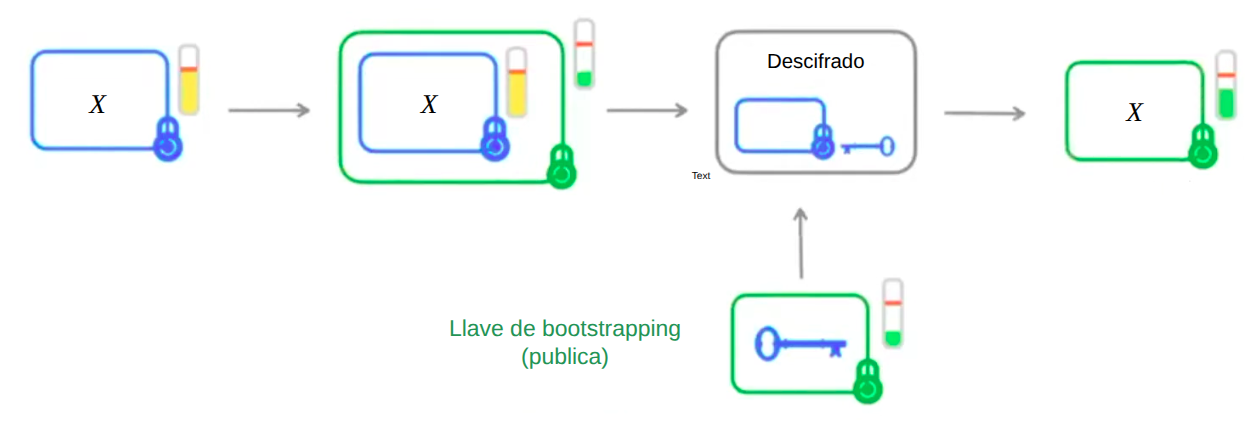
\includegraphics[width=0.7\textwidth]{bootstrap.png}
        \caption{Diagrama esquemático del proceso de Bootstrapping.}
    \end{figure}
\end{frame}

% --- Part 4: Redes Neuronales y Cifrado Homomórfico ---
\section{Redes Neuronales y FHE}
\SectionFrame{Redes Neuronales y Cifrado Homomórfico}

\begin{frame}{Operaciones en el espacio cifrado}
    La ejecución de RNAs sobre FHE requiere traducir las operaciones tensoriales al dominio de polinomios:
    \vspace{0.4cm}
    \begin{itemize}
        \setlength{\itemsep}{12pt}
        \item \textbf{Multiplicación Matriz-Vector:} Se realiza mediante la técnica de diagonalización desarrollada por Halevi y Shoup.
        \item \textbf{Convoluciones:} Se transforman en productos matriciales eficientes mediante la técnica \textbf{Im2Col} sobre los datos cifrados.
        \item \textbf{Funciones de Activación:} Dado que FHE solo permite sumas y productos, activaciones como ReLU o Sigmoid se sustituyen por \textbf{aproximaciones polinomiales} (ej. $f(x) = x^2$).
    \end{itemize}
\end{frame}

\begin{frame}{Redes de interés}
    \begin{itemize}
        \item \textbf{Capa Lineal ($y = Wx + b$):} Base de los Perceptrones Multicapa (MLP), resolvemos mediante productos punto paralelos.
        \item \textbf{Capa Convolucional:} Fundamental para visión artificial, procesa regiones espaciales locales.
    \end{itemize}
    \vspace{0.2cm}
    \begin{columns}[t]
        \column{0.45\textwidth}
        \centering
        \begin{tikzpicture}[scale=0.55, every node/.style={font=\tiny}]
            % Input layer
            \foreach \i in {1,...,3}
                \node[circle, draw, fill=blue!20] (I\i) at (0,\i) {};
            % Hidden layer
            \foreach \i in {1,...,4}
                \node[circle, draw, fill=orange!20] (H\i) at (1.5,\i-0.5) {};
            % Output layer
            \foreach \i in {1,...,2}
                \node[circle, draw, fill=green!20] (O\i) at (3,\i+0.5) {};
            % Connections
            \foreach \i in {1,...,3}
                \foreach \j in {1,...,4}
                    \draw[->, gray!60] (I\i) -- (H\j);
            \foreach \i in {1,...,4}
                \foreach \j in {1,...,2}
                    \draw[->, gray!60] (H\i) -- (O\j);
            \node[below=0.2cm] at (1.5, 0.5) {Estructura MLP};
        \end{tikzpicture}
        
        \column{0.55\textwidth}
        \centering
        \begin{tikzpicture}[scale=0.5, every node/.style={font=\tiny}]
            % ENTRADA
            \begin{scope}[shift={(0,0)}]
                \draw[step=0.6cm, gray!60, thin] (0,0) grid (1.8,1.8);
                \fill[blue!20, opacity=0.5] (0,0.6) rectangle (1.2,1.8);
                \node[below] at (0.9, 0) {Entrada};
            \end{scope}
            % KERNEL
            \begin{scope}[shift={(2.5,0.3)}]
                \draw[step=0.6cm, gray!60, thin] (0,0) grid (1.2,1.2);
                \fill[orange!20, opacity=0.5] (0,0) rectangle (1.2,1.2);
                \node[below] at (0.6, 0) {Kernel};
            \end{scope}
            \draw[->, thick, gray!60] (1.9, 0.9) -- (2.4, 0.9);
            \draw[->, thick, gray!60] (3.8, 0.9) -- (4.3, 0.9);
            % SALIDA
            \begin{scope}[shift={(4.5,0.6)}]
                \draw[step=0.6cm, gray!60, thin] (0,0) grid (0.6,0.6);
                \fill[green!20] (0,0) rectangle (0.6,0.6);
                \node[below] at (0.3, 0) {Salida};
            \end{scope}
            \node[below=0.2cm] at (2.5, -0.5) {Operación Convolucional};
        \end{tikzpicture}
    \end{columns}
\end{frame}

% --- Part 5: Problemática y Propuesta ---
\section{Problemática y Propuesta}
\SectionFrame{Problemática y Propuesta}

\begin{frame}{Limitaciones Actuales}
    A pesar de la madurez de CKKS, existe una brecha crítica entre la teoría y la aplicación real en RNAs:
    \vspace{0.3cm}
    \begin{itemize}
        \setlength{\itemsep}{12pt}
        \item \textbf{Limitado por CPU:} Las bibliotecas de CKKS más robustas son extremadamente lentas al escalar a modelos complejos debido a su dependencia de la CPU.
        \item \textbf{Incompatibilidad de GPU:} Herramientas actuales aceleradas por GPU no usan CKKS, limitando la precisión de los modelos.
        \item \textbf{Falta de herramientas:} Ausencia de bibliotecas que permitan construir modelos de redes neuronales abstrayendo la complejidad técnica de FHE para el desarrollador.
    \end{itemize}
\end{frame}

\begin{frame}{Objetivos}
    \textbf{Objetivo General:}
    \begin{itemize}
        \item Desarrollar una biblioteca de código abierto en Python para el cómputo de operaciones tensoriales, utilizando el esquema CKKS y aprovechando la GPU.
    \end{itemize}
    \vspace{0.2cm}
    \textbf{Objetivos Específicos:}
    \begin{itemize}
        \item Diseñar una interfaz en Python para interactuar con FIDESlib y OpenFHE.
        \item Implementar módulos para operaciones de tensores y matrices, abstrayendo la complejidad de CKKS.
        \item Crear casos de uso para inferencia privada en modelos de aprendizaje automático.
        \item Comparar el rendimiento frente a otras bibliotecas de cifrado homomórfico.
    \end{itemize}
\end{frame}

\begin{frame}{Tecnologías}
    \begin{itemize}
        \setlength{\itemsep}{10pt}
        \item \textbf{Python y CUDA:} Lógica de alto nivel en Python y optimización de operaciones no nativas en CUDA.
        \item \textbf{FIDESlib:} Implementación eficiente del esquema CKKS acelerada por GPU.
        \item \textbf{OpenFHE-Python:} Puente principal (\textit{bindings}) para la gestión de las primitivas criptográficas.
        \item \textbf{Pybind11:} Creación de \textit{bindings} personalizados para la comunicación eficiente entre C++ y Python.
    \end{itemize}
\end{frame}

\begin{frame}{Evaluación y Comparativa}
    Se comparará la biblioteca propuesta frente a \textbf{TenSEAL} (CKKS en CPU) y \textbf{Concrete ML} (TFHE en GPU) utilizando modelos de referencia (MLP y CNN) bajo los siguientes criterios:
    \vspace{0.3cm}
    \begin{itemize}
        \setlength{\itemsep}{12pt}
        \item \textbf{Precisión Numérica:} Medir el impacto de las aproximaciones polinomiales y la gestión del ruido frente a modelos en texto plano. Se evaluará la efectividad de los modelos dado el error introducido por las operaciones cifradas.
        \item \textbf{Rendimiento computacional:} Evaluación del tiempo de ejecución y el uso de memoria (RAM/VRAM) para cuantificar la eficiencia de la aceleración por GPU.
    \end{itemize}
    \vfill
    \begin{center}
        \small La biblioteca será publicada de forma abierta en un repositorio público (GitHub).
    \end{center}
\end{frame}

% --- Part 6: Proposed GPU Library (Slides 22-26) ---
\section{Propuesta de Trabajo}

\begin{frame}{Limitaciones de las Herramientas Actuales}
    \begin{itemize}
        \item Bibliotecas como SEAL, HELib o PALISADE usan solo CPU.
        \item El cómputo homomórfico es intensivo; la CPU es un cuello de botella.
        \item Necesidad de aceleración por hardware para modelos complejos.
    \end{itemize}
\end{frame}

\begin{frame}{Stack Tecnológico}
    \begin{itemize}
        \item \textbf{FIDESlib:} Backend optimizado en CUDA/C++.
        \item \textbf{OpenFHE-Python:} Interfaz de alto nivel.
        \item \textbf{Pybind11:} Bindings para exponer C++ en Python.
    \end{itemize}
\end{frame}

\begin{frame}{Objetivos del Trabajo}
    \begin{itemize}
        \item Desarrollar una biblioteca Python para tensores cifrados en GPU.
        \item Abstraer la complejidad criptográfica del usuario.
        \item Habilitar inferencia privada de modelos reales.
    \end{itemize}
\end{frame}

\begin{frame}{Casos de Uso y Benchmarking}
    \begin{itemize}
        \item Implementación de redes DNN y CNN cifradas.
        \item Comparar contra TenSEAL (CPU) y Concrete ML (GPU-TFHE).
        \item Evaluar impacto de funciones de activación y parámetros.
    \end{itemize}
\end{frame}

\begin{frame}{Resumen y Trabajo Futuro}
    \begin{itemize}
        \item Reducción de la brecha entre criptografía y Machine Learning.
        \item Provisión de herramientas para computación privada eficiente.
        \item Extensión a modelos iterativos y procesamiento en tiempo real.
    \end{itemize}
\end{frame}


% Diapositiva Final
\begin{frame}
    \centering
    \Huge ¿Preguntas?
    \vfill
    \large \textbf{Contacto:} \\ rafael.contreras@ciens.ucv.ve
\end{frame}

\end{document}
